\documentclass[12pt]{article}

\usepackage[portuguese]{babel}
\usepackage[utf8]{inputenc}
\usepackage{amsmath}
\usepackage{commath}
\usepackage[alf]{abntex2cite}
\usepackage{indentfirst}
\usepackage{graphicx}
\usepackage{multicol,lipsum}
\usepackage{subfig}
\usepackage{geometry}

\geometry{
	paper = a4paper,
    inner = 3cm,
    outer = 3cm,
    top = 2cm,
    bottom = 2cm
}

\begin{document}
%\maketitle

\onehalfspacing

\begin{titlepage}
	\begin{center}

		\Huge{Universidade Federal de Alagoas}\\
		\large{Instituto de Computação}\\ 
		\large{Laboratório de Computação Científica e Análise Numérica}\\ 
        \vspace{220pt}
        \textbf{\LARGE{Relatório de acompanhamento de pesquisa}}\\
		%\title{{\large{Título}}}
		\vspace{3,5cm}
	\end{center}
	
	\begin{flushleft}
		\begin{tabbing}
			Aluno: Danilo Fernandes Costa\\
			Professor orientador: Alejandro Frery\\
	\end{tabbing}
 \end{flushleft}
	\vspace{1cm}
	
	\begin{center}
		\vspace{\fill}
			 Dezembro\\
		 2018
			\end{center}
\end{titlepage}

\section{Resumo}

No presente relatório são apresentados os resultados obtidos da análise numérica da decomposição de Kennaugh.

\section{Análise númerica}

Para a análise foram utilizados dados MLC, obtidos em UAVSAR, referentes à região de Cabo Canaveral, Flórida, EUA. Para a leitura dos mesmos utilizou-se o seguinte \textit{script}.

\begin{verbatim}

read_complex_file <- function(file, nrow, ncol){
  
  complex_numbers <- matrix(
    readBin(file, double(), n = 2*nrow * ncol, size = 4, endian = "little"), 
    nrow = nrow*ncol, ncol = 2, byrow = TRUE)
  
  return( matrix( complex( 
                          real = complex_numbers[,1], 
                          imaginary = complex_numbers[,2] ), 
                  nrow = nrow, ncol = ncol, byrow = TRUE))
  
}

read_file <- function(file, nrow, ncol){
  
  return(matrix(
    readBin(file, double(), n = nrow * ncol, size = 4, endian = "little"), 
    nrow = nrow, ncol = ncol, byrow = TRUE) )
}

nrow <- 7038
ncol <- 3300

hhhv_file <- file("hhhv.mlc", "rb")
hhhv <- read_complex_file(hhhv_file, nrow = nrow, ncol = ncol)

hhvv_file <- file("hhvv.mlc", "rb")
hhvv <- read_complex_file(hhvv_file, nrow = nrow, ncol = ncol)

hvvv_file <- file("hvvv.mlc", "rb")
hvvv <- read_complex_file(hvvv_file, nrow = nrow, ncol = ncol)

hhhh_file <- file("hhhh.mlc", "rb")
hhhh <- read_file(hhhh_file, nrow = nrow, ncol = ncol)

hvhv_file <- file("hvhv.mlc", "rb")
hvhv <- read_file(hvhv_file, nrow = nrow, ncol = ncol)

vvvv_file <- file("vvvv.mlc", "rb")
vvvv <- read_file(vvvv_file, nrow = nrow, ncol = ncol)

\end{verbatim}

Após a leitura dos dados, obteve-se o vetor de Kennaugh para cada pixel da imagem através do seguinte: 

\begin{verbatim}
    
kennaugh_vector <- array(0, dim = c(nrow, ncol, 16))

kennaugh_vector[,,1] <- (hhhh+hvhv+vvvv) / 2
kennaugh_vector[,,2] <- (hhhh+hvhv-vvvv) / 2
kennaugh_vector[,,3] <- (hhhh-hvhv+vvvv) / 2
kennaugh_vector[,,4] <- (-hhhh+hvhv+vvvv) / 2
 
kennaugh_vector[,,8] <- Re(hvvv)
kennaugh_vector[,,9] <- Im(hhvv)
kennaugh_vector[,,10] <- -Im(hhhv)
    
kennaugh_vector[,,11] <- Re(hhhv)
kennaugh_vector[,,12] <- Re(hhvv)
kennaugh_vector[,,13] <- Im(hvvv)
    
kennaugh_vector[,,14] <- Re(hvvv)
kennaugh_vector[,,15] <- Im(hhvv)
kennaugh_vector[,,16] <- -Im(hhhv)

\end{verbatim}

O passo seguinte foi realizado principalmente com o objetivo de analisar a precisão das funções encontradas destinadas à normalização e ao cálculo da norma euclidiana de vetores. No que se refere à obtenção do versor de um vetor, as funções encontradas são ambas \texttt{normalize.vector}, as quais residem nas bibliotecas \texttt{ppls} e \texttt{bio3d}. Aquela presente em \texttt{bio3d}, além de operar sobre vetores, pode ser aplicada a matrizes, normalizando os vetores-coluna.

Já as funções para o cálculo de normas euclidianas são \texttt{norm} e \texttt{Norm}, onde a primeira é nativa da plataforma R e a última pertence a biblioteca \texttt{pracma}. Deve ser observado que a primeira dessas funções deve ser aplicada sobre uma matriz e que considera todos os elementos desta como as componentes de um único vetor.

O procedimento realizado consiste na amostragem de 10.000 vetores de Kennaugh seguido do cálculo da norma de seus versores utilizando as funções descritas anteriormente e análise destes resultados. O \texttt{script} que faz isso utilizando as funções \texttt{Norm} e \texttt{normalize.vector} da biblioteca \texttt{ppls} é o seguinte:

\begin{verbatim}

id1 <- sample(1:nrow, size = 10000, replace = TRUE)
id2 <- sample(1:ncol, size = 10000, replace = TRUE)

norm_kennaugh <- array(0, dim = 10000)

for (i in 1:10000) {
  versor <- normalize.vector(kennaugh_vector[id1[i], id2[i],])
  norm_kennaugh[i] <- Norm( versor )
}

#Analysis
comparation <- norm_kennaugh == 1
summary(comparation)

comparation <- (1 - .Machine$double.neg.eps*2) < norm_kennaugh &
                    norm_kennaugh < (1 + .Machine$double.eps*2)
summary(comparation)

\end{verbatim}

Para as demais combinações de funções de normalização e cálculo de norma apenas linhas referentes ao \textit{loop} são substituídas. Para a combinação das funções \texttt{norm} e \texttt{normalize.vector} da biblioteca \texttt{ppls} o trecho substituto é o seguinte:

\begin{verbatim}
    
for (i in 1:10000) {
  versor <- normalize.vector(kennaugh_vector[id1[i], id2[i],])
  norm_kennaugh[i] <- norm( as.matrix( versor ), type = "F")
}
    
\end{verbatim}

Segue o trecho substituto referente à combinação de funções \texttt{Norm} e \texttt{normalize.vector} da biblioteca \texttt{bio3d}:

\begin{verbatim}

for (i in 1:10000) {
  versor <- normalize.vector(kennaugh_vector[id1[i], id2[i],])
  norm_kennaugh[i] <- Norm( versor )
  
}
\end{verbatim}

Já o trecho substituto referente à combinação de funções \texttt{norm} e \texttt{normalize.vector} da biblioteca \texttt{bio3d} é o seguinte:

\begin{verbatim}

for (i in 1:10000) {
  versor <- normalize.vector(as.matrix(kennaugh_vector[id1[i], id2[i],]))
  norm_kennaugh[i] <- norm( as.matrix( versor ), type = "F")
}

\end{verbatim}

Para fim comparativos também analisou-se o resultado utilizando trechos substitutos os quais normalizam vetores calculando sua norma e em seguida dividindo-os pela mesma. Segue o trecho utilizando a função \texttt{Norm}:

\begin{verbatim}
for (i in 1:10000) {
  norm <- Norm(kennaugh_vector[id1[i], id2[i],])
  versor <- kennaugh_vector[id1[i], id2[i],] / norm
  norm_kennaugh[i] <- Norm( versor )
}
\end{verbatim}

Já o trecho que utiliza a função \texttt{norm} é o seguinte:

\begin{verbatim}
for (i in 1:10000) {
  norm <- norm(as.matrix(kennaugh_vector[id1[i], id2[i],]), type = "F")
  versor <- kennaugh_vector[id1[i], id2[i],] / norm
  norm_kennaugh[i] <- norm( as.matrix( versor ), type = "F")
}
\end{verbatim}

Segue o gráfico com a procentagem de normas dos versores obtidos que diferiram de 1 de acordo com a abordagem:

\begin{figure}[!h]
    \centering
    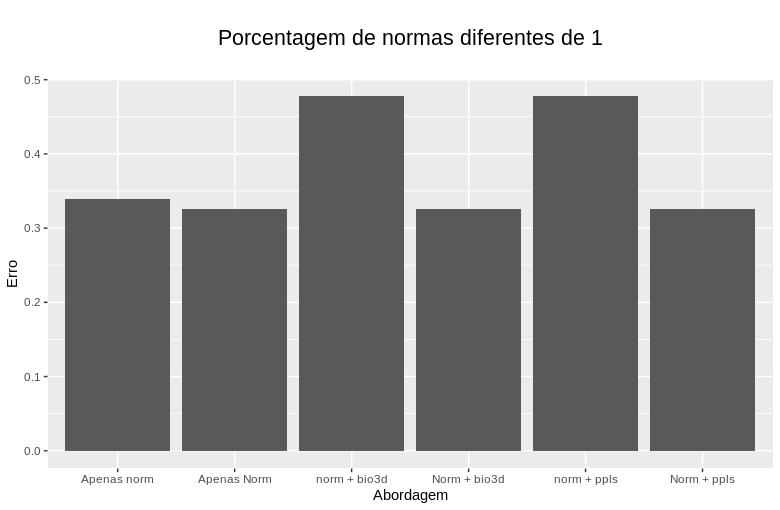
\includegraphics[width = \linewidth]{../../Figures/report_18_12_06/dif_one.png}
\end{figure}
\newpage

Segue o gráfico com a procentagem de normas dos versores obtidos que estavam fora do intervalo (1 - 2$\epsilon$, 1 + 2$\epsilon$) de acordo com a abordagem:

\begin{figure}[!h]
    \centering
    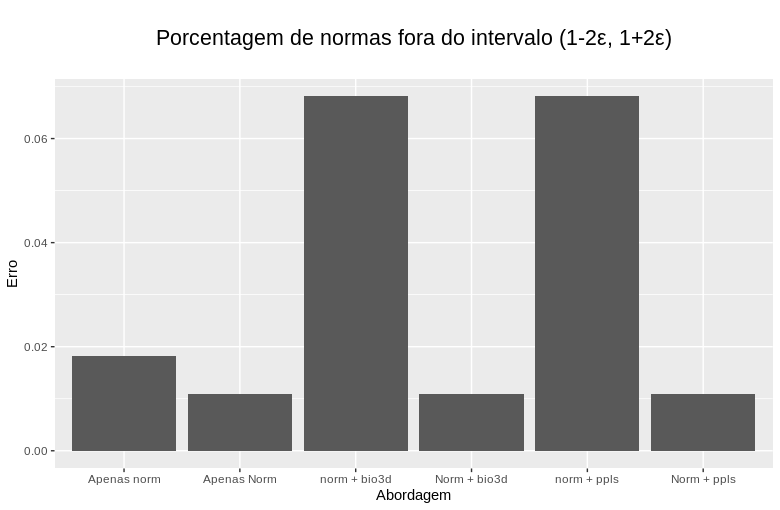
\includegraphics[width = \linewidth]{../../Figures/report_18_12_06/dif_two_eps.png}
\end{figure}

Deve ser salientado que em todas as abordagens foi utilizada a mesma amostra e o número de valores NA obtidos foi 36.

\end{document}